\documentclass[
	letterpaper, % Paper size, specify a4paper (A4) or letterpaper (US letter)
	10pt, % Default font size, specify 10pt, 11pt or 12pt
]{CSUniSchoolLabReport}

%----------------------------------------------------------------------------------------
%	REPORT INFORMATION
%----------------------------------------------------------------------------------------

\title{Frequency Components, Fast Fourier Transform, and Filtering\\ Circuits \& Signals \\ EECE2150} % Report title

\author{Michael \textsc{Brodskiy}}

\date{April 20, 2023} % Date of the report

%----------------------------------------------------------------------------------------


\begin{document}

\maketitle % Insert the title, author and date using the information specified above

\begin{center}
	\begin{tabular}{l r}
		Date Performed: & March 23, 2023 \\ % Date the experiment was performed
        Partner: & Juan \textsc{Zapata}, Oluwalaanu \textsc{Adeboye} \\ % Partner names
		Instructor: & Professor \textsc{Sun} % Instructor/supervisor
	\end{tabular}
\end{center}

\setcounter{section}{-1}

\section{Introduction}

The purpose of this laboratory experimentation was to analyze a filter mathematically and graphically through the use of a transfer function in MATLAB. This will be necessary in the future, as the construction of an electrocardiogram will require the use of filters. All generated graphs are included in the appendix.

\section{Discussion and Analysis}

\subsection{Part 1}

\subsubsection{Q1} The cutoff frequency of the given function is $15.92[\si{\hertz}]$

\subsection{Part 2}

\subsubsection{Q2 \& Q3}

\begin{center}
\begin{tabular}[h!]{|c|c|c|}
  \hline
  Frequency $[\si{\hertz}]$ & Approx. Magnitude of $H(\omega)$ $[\si{\volt}]$ & Phase Shift $[^{\circ}]$\\
  \hline
  1 & 1.8 & 90\\
  \hline
  5 & .4 & 45\\
  \hline
  10 & .2 & 25\\
  \hline
  20 & .1 & 10\\
  \hline
  100 & .01 & 1\\
  \hline
\end{tabular}
\end{center}

\subsubsection{Q4} The results do agree with our expectations

\subsection{Part 3}

\subsubsection{Q5} We recognized that, at the fundamental frequency, as well as odd integer multiples, the relative magnitude changed as the frequency increased

\subsubsection{Q6} The amplitude of the filtered signal decreased until it was zero — this was indicated by the divergence of the filtered signal from the origin

\subsubsection{Q7} The filtered time-domain waveform looks like a curved horizontal zigzag; this was expected given the frequency domain information

\subsection{Part 4}

\subsubsection{Q8\footnote{This and the next few questions are all their number here plus 3, as a few numbers were skipped in the lab}} The gain produced by the filter was -2, and the magnitudes of the filtered and unfiltered Fourier components remained unchanged

\subsubsection{Q9} The filtered signal was double the magnitude of the original signal

\subsubsection{Q10} The filtered time-domain waveform was like the filter Fourier components but had lower magnitudes; this was in line with the expected results

\subsubsection{Q11} The results agreed with what was observed in the op-amp filter lab

\section{Conclusion}

Overall, this laboratory experiment allowed for a thorough analysis of filters and their fast Fourier transforms, as, by integrating MATLAB and generating graphs, the concepts became much more visually clear. As such, filters were more easy to grasp.

\section{Appendix}

\begin{figure}[h!]
  \centering
  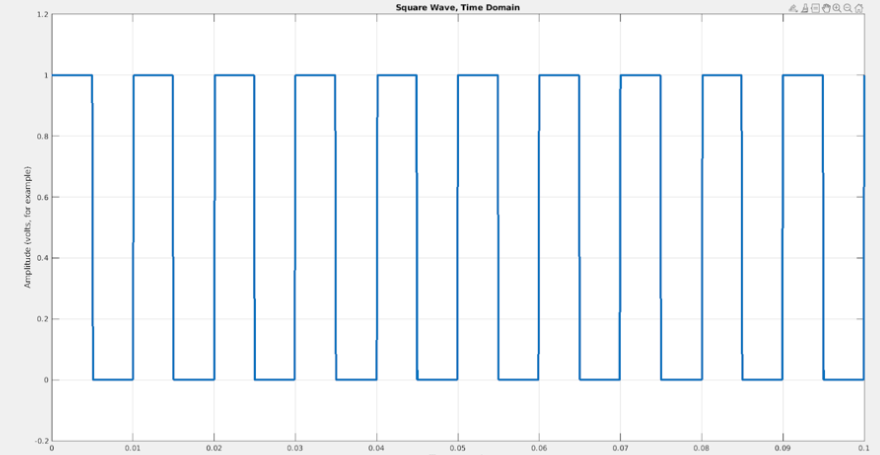
\includegraphics[width=.9\textwidth]{Figures/L13Q1.png}
  \caption{Square Wave, Time Domain}
  \label{fig:1}
\end{figure}

\begin{figure}[h!]
  \centering
  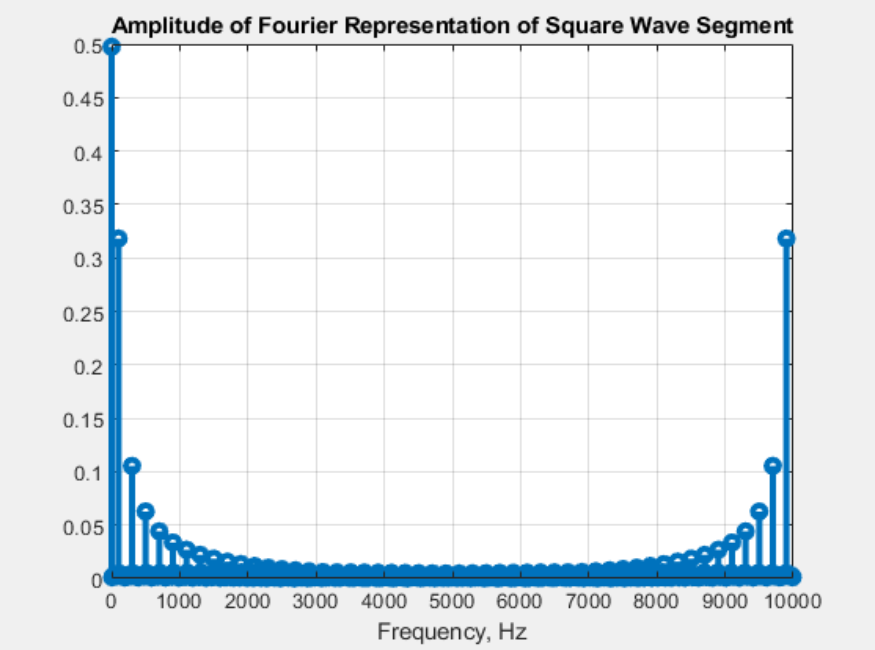
\includegraphics[width=.9\textwidth]{Figures/L13Q1-2.png}
  \caption{Amplitude of Fourier Representation of Square Wave Segment}
  \label{fig:2}
\end{figure}

\begin{figure}[h!]
  \centering
  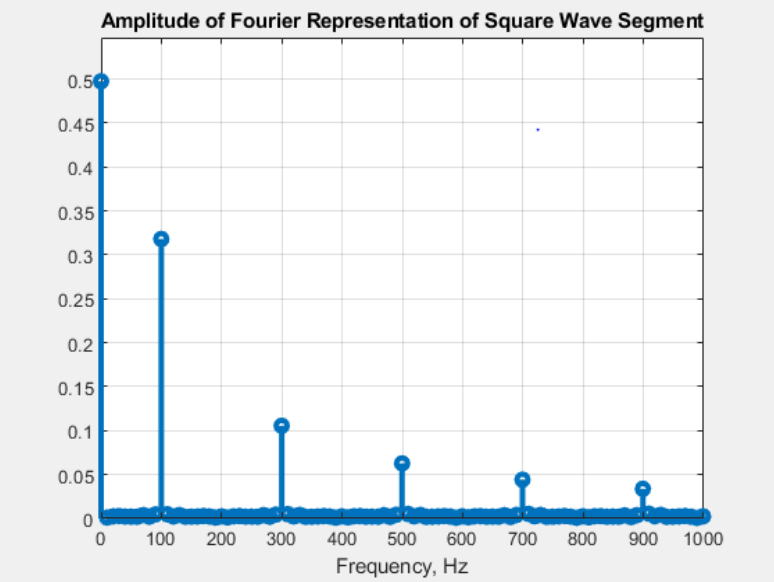
\includegraphics[width=.9\textwidth]{Figures/L13Q1-3.png}
  \caption{Amplitude of Fourier Representation of Square Wave Segment}
  \label{fig:3}
\end{figure}

\begin{figure}[h!]
  \centering
  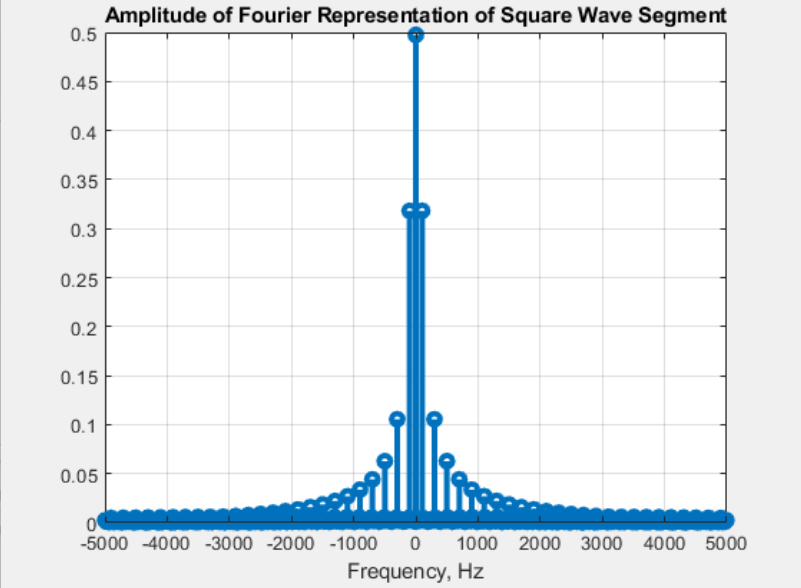
\includegraphics[width=.9\textwidth]{Figures/L13Q1-4.png}
  \caption{Amplitude of Fourier Representation of Square Wave Segment}
  \label{fig:4}
\end{figure}

\begin{figure}[h!]
  \centering
  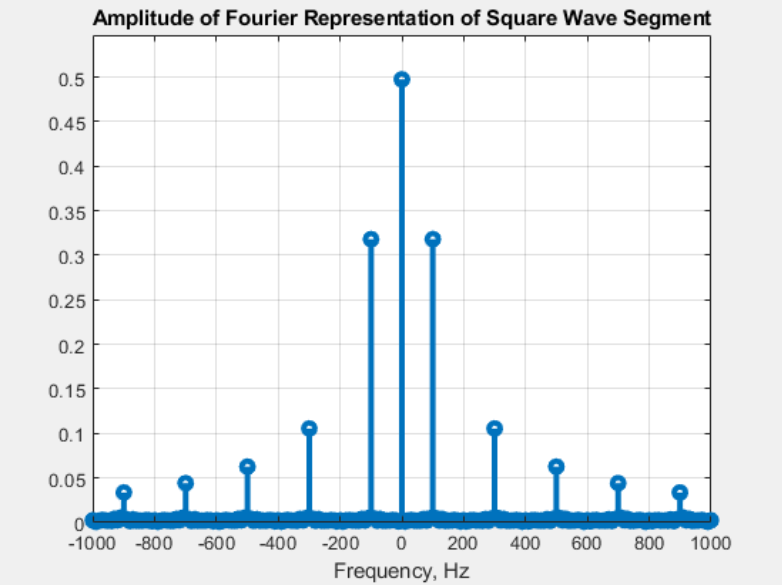
\includegraphics[width=.9\textwidth]{Figures/L13Q1-5.png}
  \caption{Amplitude of Fourier Representation of Square Wave Segment}
  \label{fig:5}
\end{figure}

\begin{figure}[h!]
  \centering
  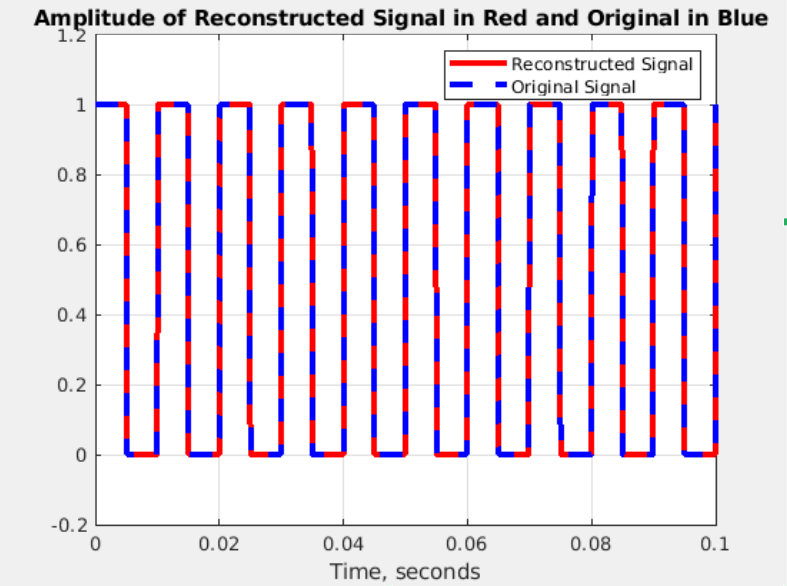
\includegraphics[width=.9\textwidth]{Figures/L13Q1-6.png}
  \caption{Amplitude of Reconstructed Signal in Red and Original in Blue}
  \label{fig:6}
\end{figure}

\begin{figure}[h!]
  \centering
  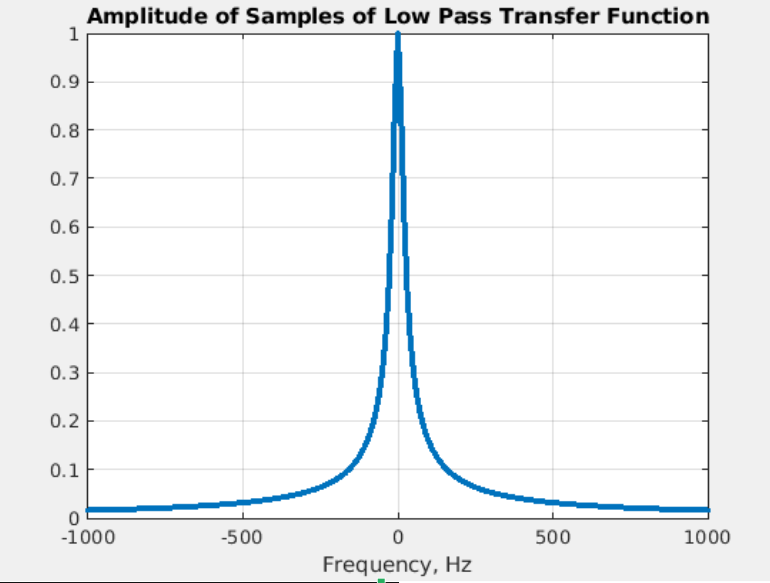
\includegraphics[width=.9\textwidth]{Figures/L13Q1-7.png}
  \caption{Amplitude of Samples of Low Pass Transfer Function}
  \label{fig:7}
\end{figure}

\begin{figure}[h!]
  \centering
  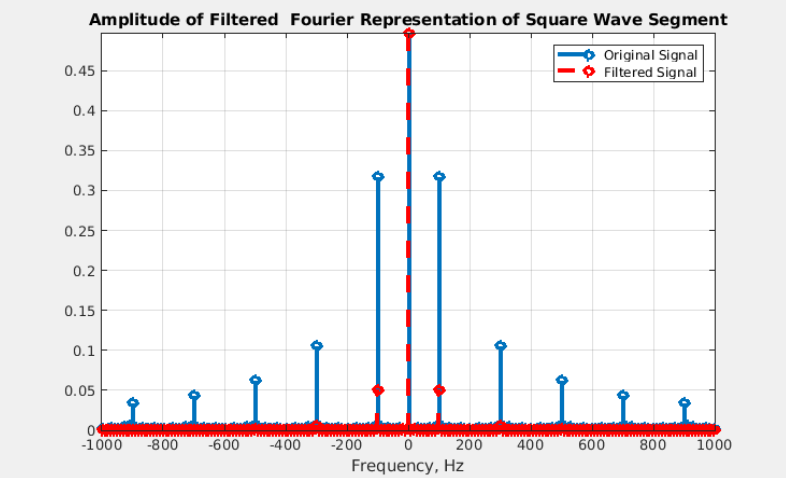
\includegraphics[width=.9\textwidth]{Figures/L13Q1-8.png}
  \caption{Amplitude of Filtered Fourier Representation of Square Wave Segment}
  \label{fig:8}
\end{figure}

\end{document}
